	\documentclass[twoside]{article}
\usepackage{../../estilo-ejercicios}

%--------------------------------------------------------
\begin{document}

\title{Relación 1}
\author{Javier Aguilar Martín}
\maketitle


\begin{ejercicio}{3.1}
Compute the chromatic number of the following graphs:

\begin{figure}[h!]
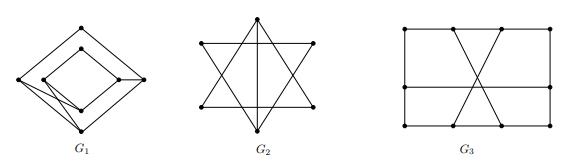
\includegraphics[scale=0.7]{grafos31}
\end{figure}
\end{ejercicio}
\begin{solucion}
$\chi(G_1)=2$ (empezar dando colores 1 y 2 a los de más abajo a la izquierda). Como $G_2$ contiene $K_3$, $\chi(G_2)\geq 3$. Como además es tripartido tenemos la desigualdad opuesta, así que $\chi(G_2)=3$. $\chi(G_3)=2$ (empezar dando colores 1 y 2 a los del medio). 
\end{solucion}

\newpage


\begin{ejercicio}{3.2}
Which of the following hold true?
\begin{enumerate}[a)]
\item For every $n ≥ 4$ there exists a planar graph $G$ with $n$ vertices and chromatic
number $χ(G) = 4$.
\item If $χ(G) ≤ 4$ then $G$ is planar.
\item There exists a graph $G$ with $χ(G) = 3$ and independence number 5.
\end{enumerate}
\end{ejercicio}
\begin{solucion}\
\begin{enumerate}[a)]
\item es cierto porque basta partir de $K_4$, que es planar, y añadir vértices aislados.
\item falso, $\chi(K_{3,3})=2$. 
\item cierto, $K_{5,5,5}$.  
\end{enumerate}

\end{solucion}

\newpage

\begin{ejercicio}{3.3}
 Show that there is no graph of order 6, size 13, and chromatic number 3.
\end{ejercicio}
\begin{solucion}
El grafo $G$ que se pide es el resultado de eliminar 2 aristas en $K_6$, ya que $\binom{6}{2}=15$. Si se eliminan dos aristas incidentes, el grafo resultante contiene a $K_5$, y si se eliminan dos aristas no incidentes el resultado contiene a $K_4$. En cualquier caso, $\chi(G)>3$. 
\end{solucion}

\newpage

\begin{ejercicio}{3.4}

At a gathering of eight employees of a company, which we denote by $A = \{a_1, a_2, \dots , a_8\}$,
it is decided that it would be useful to have these individuals meet in committees of three
to discuss seven issues of importance to the company. The seven committees selected
for this purpose are:
$$A_1 = \{a_1, a_2, a_3\}, A_2 = \{a_2, a_3, a_4\}, A_3 = \{a_4, a_5, a_6\}, A_4 = \{a_5, a_6, a_7\}$$

$$A_5 = \{a_1, a_7, a_8\}, A_6 = \{a_1, a_4, a_7\}, A_7 = \{a_2, a_6, a_8\}$$
If each committee is to meet during one of the time periods

1-2 pm, 2-3 pm, 3-4 pm, 4-5 pm, 5-6 pm,

what is the minimum number of time periods needed for all seven committees to meet?

\end{ejercicio}
\begin{solucion}



\end{solucion}

\newpage

\begin{ejercicio}{3.5}

There are nine courses $A1,\dots, A9$ in the first year of the Degree in Computer Science.
There are students who are taking simultaneously courses $A1$ and $A2$; $A3$ and $A4$; $A5$
and $A6$; $A7$ and $A8$. In addition, every student that is taking a course among $A1,\dots, A8$
has to take also course $A9$. Design a schedule containing the minimum number of time
periods so that students can attend to all their courses.

\end{ejercicio}
\begin{solucion}
 
 
\end{solucion}

\newpage

\begin{ejercicio}{3.6}
Show that for the cycle $C_n$ of length $n$, $P(C_n; λ) = (λ − 1)^n + (−1)^n
(λ − 1)$, $n ≥ 3$
\end{ejercicio}
\begin{solucion}
Para $n=3$, como $C_3=K_3$, es fácil comprobar que $P(C_3;\lambda)=\lambda(\lambda-1)(\lambda-2)=(λ − 1)^3 −(λ − 1)$. Para $n>3$ usamos la fórmula recursiva del polinomio cromático, teniendo en cuenta que en un ciclo ninguna arista es un puente. Asumimos como hipótesis de inducción que el resultado es cierto para $C_{n-1}$. Entonces, 
\[
P(C_n;\lambda)=P(C_n-e;\lambda)-P(G/e;\lambda)=P(P_n;\lambda)-P(C_{n-1};\lambda)=
\]
\[
\lambda(\lambda-1)^{n-1}-(λ − 1)^{n-1} - (−1)^{n-1}(λ − 1)=(λ − 1)^{n-1}(\lambda-1)-(−1)^{n-1}(λ − 1))
\]
\[
=(λ − 1)^n+(−1)^n(λ − 1).
\]


%\textbf{ALTERNATIVA}
%
%Usando el ejercicio siguiente, partimos de que existe un $K_3$ monocromático, digamos azul, por ejemplo en los vértices $v_1,v_2,v_3$. Supongamos que de $v_1,v_2,v_3$ salen 2 aristas azules hacia $v_3,v_4,v_5$, entonces podemos encontrar un 4-ciclo monocromático. En otro caso, al menos dos aristas de $v_4,v_5,v_6$ al $K_3$ son rojas, de donde sacamos el 4-ciclo rojo. 
\end{solucion}

\newpage

\begin{ejercicio}{3.7}
Show that there is no graph with the following polynomials as chromatic polynomials:
(i) $λ^5 − 4λ^4 + 8λ^3 − 4λ^2 + λ$; (ii) $λ^7 − λ^6 + 1$.
\end{ejercicio}
\begin{solucion}
\begin{enumerate}[(i)]
\item Conexo. El 1 no es raíz así que no tiene bloques, pero eso quiere decir que no contiene ningún $K_2$, por lo que solo podría ser un vértice, que no tiene ese polinomio cromático. 

Esto no es del ejercicio pero me salió al interpretar mal una cosa y puede ser útil: Solo hay 3 árboles de 4 aristas: $P_5$, el grafo estrella y un árbol con un punto de corte de orden 2. Todos ellos tienen como polinomio cromático
\item $a_0=1\neq 0$. 
\end{enumerate}
\end{solucion}

\newpage

\begin{ejercicio}{3.8}
Find a graph $G$ whose chromatic polynomial is $λ^5 − 6λ^4 + 11λ^3 − 6λ^2$
.
\end{ejercicio}
\begin{solucion}
Tiene que ser un grafo de 5 vértices, 6 aristas, 2 componentes conexas y con 1 bloque. Como tiene dos componentes conexas y un solo bloque, tiene un vértice aislado, así que las 6 aristas restantes están concentradas en los otros 4 vértices. Necesariamente debe ser entonces un $K_4$ el resto del grafo. El polinomio cromático del grafo que hemos descrito es $\lambda^2(\lambda-1)(\lambda-2)(\lambda-3)=λ^5 − 6λ^4 + 11λ^3 − 6λ^2$.



\end{solucion}
\newpage

\begin{ejercicio}{3.9}
Let $P(G, λ) = \sum^n_{i=0} a_iλ^i$ be the chromatic polynomial of a graph $G$ with $n$ vertices and
$m$ edges. Prove that $a_0 = 0$, $a_n = 1$, and $a_{n−1} = −m$.
\end{ejercicio}
\begin{solucion}

\end{solucion}

\newpage

\begin{ejercicio}{3.10}
Let $G$ be a simple graph with $n$ vertices. Show that $G$ is a tree if and only if $P(G, λ) =
λ(λ − 1)^{n−1}$.

\end{ejercicio}
\begin{solucion}
\end{solucion}

\newpage

\begin{ejercicio}{3.11}
 Prove that $C_4$ and $K_5$ are chromatically unique. Extend the argument to $C_n$ and $K_n$.
\end{ejercicio}
\begin{solucion}
En el caso de $K_n$, cualquier grafo con $n$ vértices y $\binom{n}{2}$ aristas tiene que ser isomorfo a $K_n$. Para $C_n$, un grafo de $n$ vértices y $n$ aristas con girth $C_n$ tiene que ser necesariamente $C_n$. 
\end{solucion}

\newpage

\begin{ejercicio}{3.12}
Two chromatically equivalent graphs $G$ and $H$ have the same order, the same size, and
the same chromatic number. Show that the converse of this statement is false.
\end{ejercicio}
\begin{solucion}
Si tienen el mismo polinomio cromático tienen el mismo orden (grado del polinomio), tamaño (es uno de los coeficientes) y el mismo número cromático (mínimo natural para el que el polinomio es positivo). Dos grafos no cromáticamente equivalentes que comparten todas estas características son \url{https://math.stackexchange.com/questions/3024221/find-two-graphs-with-same-order-size-and-chromatic-number-but-with-different-c/3024250#3024250}
\end{solucion}

\end{document}
